
%\begin{abstract}
%When developing predictors for machine learning applications, practitioners often want to have simple and working predictors early and continue to improve them with available computational resources. 
%In this work, we propose a neural architecture search (NAS) algorithm that iteratively augments existing networks by adding shortcut connections and layers. At each iteration, we greedily select among the most cost-efficient models a parent model, and insert into it a number of candidate layers.  To learn which combination of additional layers to keep,  we simultaneously train their parameters and select the most promising candidates via feature selection techniques. The selected candidates are then jointly trained with the parent model.  Within 15 GPU-days, the proposed network growth NAS algorithm (\Petridish) can already find a model on CIFAR-10 that achieves 2.79\% error rate using 2.8M parameters.  We also transfer the model to ILSVRC2012, and it achieves 25.4\% top-1 error rate using 6.2M parameters and 810M multiply-adds. 
%Furthermore, unlike recent studies of NAS that almost exclusively focus on the small search space of repeatable network modules (cells), this work also shows that a direct search among the more general networks (macro) can also find cost-effective models when macro search is allowed to start with the same initial models as cell search does. 
%\end{abstract}

\section{Introduction}
\label{sec:nas_introduction}

Deep neural networks have achieved state-of-the-art performance on many large scale supervised learning tasks across many domains like computer vision, natural language processing and audio and speech-related tasks. But most gains have come from manually designed architectures which have inspired further improvements via careful experimentation coupled with significant experience and intuition of a skilled practitioner. Such skilled practitioners usually have significant domain knowledge of the task at hand that allows them to make rapid progress. But the fact remains that the task of designing a deep network architecture from scratch remains mostly a game of trial and error. As a consequence there has been significant effort in the community to address this issue via attempts to design algorithms that automatically find good architectures and informally referred to as AutoDNN and/or Neural Architecture Search (NAS) \cite{nas}. 

NAS literature can be broadly categorized along three main dimensions: 1. search space 2. search procedure and 3. performance estimation strategy during the search procedure. The search space can be broadly further divided to methods that search either 1. a more general space of architectures often termed as macro-search or 2. a more constrained search space called micro or cell-search. In cell-search a good outer skeleton is often assumed. For example in image classification datasets it is common to often assume either ResNet~\citep{resnet} or DenseNet~\cite{densenet} style outer skeletons. The search can then be restricted to finding cells that fill in the slots in the outer skeleton so that the overall architecture has good performance. Cell-search is much more popular due to a number of reasons: 1. One can leverage domain knowledge of experts who have painstakingly come up with good architectures and focus the search to a smaller space. 2. Transfer to larger datasets where more capacity is often needed can be obtained by trivially stacking many cells to create larger networks. The very aspects that make cell-search attractive also prevent it from providing a truly general solution: when good outer skeletons are not available for novel domains/datasets or there is reason to believe that significant performance is left on the table, cell-search cannot be applied. By restricting the search space it is quite possible that significant performance is left on the table. On large datasets in production environments this feature is especially important. Macro-search in principle doesn't suffer from any of the above limitations but suffers from searching a much more general and larger architecture space. 

In this work we propose a method for growing networks from small to large where we opportunistically add layers inspired by the ``cascade correlation'' work of \cite{cascadecorr}. We term our approach \Petridish. \Petridish can be used with both macro and cell-search spaces. Importantly \Petridish achieves better performance on macro search spaces than any other NAS algorithm which considers macro search results. Furthermore the final results achieved by \Petridish macro are comparable to those of the current best cell-search methods including that of \Petridish cell-search methods.

\begin{itemize}
\item We propose an approach to increase complexity of neural networks during training iteratively. We alternate between two phases. The first expands the model with potential shortcut connections and train them jointly. The second phase trim the previous potential connections using feature selection and continue training the model. 
\item The proposed approach can be applied to both improve a small repeatable pattern, called cell, and improve the macro network architecture directly, unlike most popular approaches that only focus on cells. This opens up neural architecture search to fields where no domain knowledge of the macro structure exists. 
\item On cell-search, the proposed method finds a model that achieves 2.61\% error rate on CIFAR10 using 2.9M parameters within 5 GPU-days. 
The model achieves 26.0\% error rate on ILSVRC2012 using 4.8M parameters and 598M multi-adds.
\item On macro-search, the proposed method finds a model that achieves 2.83\% error rate on CIFAR10 using 2.2M parameters within 5 GPU-days. 
%The model achieves \% error rate on ILSVRC2012 using M parameters and M multi-adds.
\item The proposed approach can warm start from existing networks, leveraging previous training results. Furthermore, it directly expands models on the lower convex hull of error rate vs. flops and is hence able to naturally produce a gallery of cost-effective models which is critical for production serving needs. 
\end{itemize}


\section{Related Works}
\label{sec:nas_background}
%\begin{itemize}
%    \item Cascade-correlation
%    \item NAS. (RL. EA. Gradient based.) 
%    \item (Micro. Macro.) 
%    \item Multi objective NAS; Pareto Front Nas 
%    \item Evaluation with few epochs vs many epochs
%    \item Incremental training, AdaNet, Boosted ResNet, Net morphism
%    \item Test~\cite{nas, NASCell, Hsu2018MONASMN, Elsken2018NeuralAS, Real2018RegularizedEF, Liu2018DARTSDA, Kandasamy2018BNAS, Pham2018EfficientNA, Liu2017ProgressiveNA}
%\end{itemize}

One of the earliest architecture search work was by \cite{cascadecorr} termed the ``Cascade-Correlation Learning Architecture'' (C2) which has inspired \Petridish. In C2 the search begins with a minimal network which is trained by any routine training algorithm like backpropagation with stochastic gradient descent. Once training error saturates C2 considers adding a candidate hidden neuron. The candidate hidden neuron before insertion to the network is connected to the input neurons and all currently existing hidden neurons. The weights of the incoming connections to this shadow neuron are optimized such that the correlation between the activations of this shadow neuron and the error at the output neurons is maximized. Then the shadow neuron is inserted into the network and its incoming weights are frozen. Its outgoing weights are then trained in the usual way. There are various similarities between C2 and \Petridish which we discuss in Sec.~\ref{sec:soft_vs_hard}.
C2 is also one of the first works that studies the idea of gradually expanding neural networks during training. This idea was studied recently by~\citep{adanet, boostedresnet} through the view of boosting small networks in the context of modern networks. 

The work of \citep{nas,NASCell} renewed interest in NAS in recent times. Their method uses a recursive neural network (RNN) as a controller network which is used to sample architectures. Each of these architectures are trained on separate machines and their resulting accuracies are used to update the parameters of the controller network via policy gradients~\citep{policygradient}. The majority of the time is spent in training each of the sampled architectures in parallel on independent machines. The resulting search times are generally on the order of thousands of GPU hours (See Table~\ref{tab:cifar10_search}). \cite{Pham2018EfficientNA} introduced a much more efficient version of this algorithm termed as Efficient Neural Architecture Search (ENAS) where the controller samples network architectures from a large super-graph of all possible architectures but trains them all jointly where the weights of edges which are common amongst the sampled architectures are shared across all of them at training time. This leads to orders of magnitude improvement in search times but still has the restriction that a super-graph to sample from must be constructed apriori.
\cite{Liu2017ProgressiveNA} proposed a method which instead of using policy gradients as in \cite{NASCell}, trains predictors on the results of training a batch of architectures to predict top-K architectures which are likely to do well in subsequent rounds in a progressive manner and hence termed as Progressive Neural Architecture Search (PNAS). 
\cite{Liu2018DARTSDA} proposed a novel method based on bilevel optimization~\citep{bilevel_opt} termed as Differentiable Architecture Search (DARTS) which relaxes the originally discrete optimization problem to a continuous one and maintains two sets of continuous parameters: 1. The (architecture) parameters over the layer types and 2. The regular parameters of the network itself for each layer type. This is optimized in an alternating fashion where first the architecture parameters are trained alternated by the parameters of the layers of each type. Discrete architectures are then backed out by just selecting the architecture parameters which have the maximum value and discarding others. DARTS achieves impressive results on cell-search space with short search times.
\cite{Elsken2018EfficientMN, CaiPathLevel} proposed an alternative insight to speed up search by incrementally evolving models from existing cost-effective models. In particular,~\cite{Elsken2018EfficientMN} explore expanding the Pareto-frontier, a set of points that do not have strict superior points, of the parameter-versus-accuracy plot to find parameter-efficient models. We refer the reader to the excellent survey article by \cite{Elsken2018NeuralAS} for more details on this rapidly evolving field. 


\section{Neural Architecture Search as Optimization}

Given a data sample $x$ with label $y$, a neural network architecture $\alpha$ with parameters $w$ produces 
a prediction $\hat{y}(x ; \alpha, w)$ and suffers a prediction loss $\ell(\hat{y}(x ; \alpha, w), y)$.
The empirical training loss is then 
\begin{align}
\mathcal{L}(\alpha, w) = \mathbb{E} _{x, y \sim \mathcal{D}} [ \ell(\hat{y}(x ; \alpha, w), y) ] ,
\end{align}
where $\mathcal{D}$ is the empirical training data. 
Then the problem of neural architectures search can be formulated as a bi-level optimization~\citep{bilevel_opt}
of both the network architecture $\alpha$ and the model parameters $w$ under the expected training loss $\mathcal{L}$ 
as follows.
\begin{align}
\min _{\alpha} \mathcal{L} (\alpha, w(\alpha)),
\quad
s.t. \quad w(\alpha) = \argmin _w \mathcal{L} (\alpha, w) 
\quad and \quad c(\alpha) \leq K,
\label{eq:bilevel_nas}
\end{align}
where $c(\alpha)$ represents the test-time computational cost of the architecture, and $K$ is some constant. 

We formalize $\alpha$ as a set of discrete decisions on which operations to include in an architecture.
Let $x_1, x_2,...,$ be intermediate layers, and $x_0 = x$ is the input. Each layer $x_i$ is a function
of the previous layers, i.e., $x_{i} = f_i ( x_0, x_1,..., x_{i-1})$ for some function $f_i$, 
though it is not necessary for $x_i$ to directly use each of the previous layers.
Each shortcut connection is defined by a triple $(x_{j}, x_{i}, op)$, 
where $x_j$ and $x_i$ ($j < i$) represent the input and output layers, and $op$ is a unary operation such 
as conv 3x3 and max pooling 3x3. Such a shortcut results in a tensor $op(x_{j})$ that can be used directly by 
$x_i$. Shortcuts to $x_i$ are combined by a merge operation 
at $x_i$, such as averaging, summation, or concatenation in order to form $x_i$.
In this work, we set the merge operations with ablation studies. 
Instead, we focus on the choice of the shortcut connections, i.e., each $\alpha$ is 
an unordered collection of $(x_j, x_i, op)$. 

                   
                   
                   
                                                                         
\subsection{Connection to Feature Selection}

Before delving into a proposed approach, we first draw an interesting connection of Eq.~\ref{eq:bilevel_nas}
to a well studied problem, feature selection for linear predictions, whose optimization formulation follows.
\begin{align}
&\min _{\alpha} \frac{1}{2n} \Vert Y - X_{\alpha} w(\alpha) \Vert ^2 + \frac{\lambda}{2} \Vert w \Vert ^2 \\
&s.t. \quad w(\alpha) = (\frac{1}{n}X_{\alpha}^TX_{\alpha} + \lambda I)^{-1} \frac{1}{n} X_{\alpha}Y 
\quad and \quad c(\alpha) \leq K,
\label{eq:bilevel_gomp}
\end{align}
where $X \in \mathcal{R}^{n \times d}$ is the feature matrix of the $n$ samples of $d$-dimensional features,
$Y \in \mathcal{R}^n$ is the regression targets, and $X_{\alpha}$ selects the features included in $\alpha$.
We note that Eq.~\ref{eq:bilevel_nas} generalizes Eq.~\ref{eq:bilevel_gomp}, since $w(\alpha)$ solves for the 
optimal coefficient given the selected features.

This observation permits us to translate between existing NAS algorithm to the feature selection problem. 
In particular,~\citep{nas,Real2017EvoNet} apply reinforcement learning and evolutionary algorithm to 
guide the trials of architecture $\alpha$, and train the potential architectures independently. 
Such methods, when applied to feature selection, are equivalent to exploring all subset of features 
using reinforcement learning or evolutionary algorithms. As a result, it is understandable that
they search for thousands of GPU-days. 

In contrast, the more recent works~\citep{Pham2018EfficientNA,Liu2018DARTSDA} train all possible
networks at the same time by training the super-graph that contains all possible shortcut connections.
Then they train at the same time a selection procedure to select the most promising 
sub-graph from this super-graph. Such procedures draw parallel to backward elimination 
and sparse optimization for feature selection, 
where the irrelevant features are iteratively removed or down-weighted. 

Besides exhaustive search, sparse optimization and backward elimination, there is another popular branch of approaches 
for feature selection, forward selection, where feature are iteratively selected, or their coefficients are gradually increased. 
Unfortunately, common algorithms such as 
Forward Regression (FR) and its approximation Orthogonal Matching Pursuit (OMP),
cannot 
directly be applied to the NAS problem, because both methods require computing 
$w(\alpha)$ at each architecture, and such computation takes a GPU-day on its own. Instead, we have
to consider methods that approximate $w(\alpha)$ and $\alpha$ at the same time. Fortunately,
one such forward algorithm for feature selection is Least-angle regression (LARS)~\citep{lars}. 

In LARS, we compute the correlation between the residual of linear prediction and
each feature, and find the feature with the largest absolute correlation. Then we update the 
coefficient of this feature until its absolute correlation is no longer the largest.
One practical approximation of LARS is to iteratively update the coefficients of the most 
correlated feature with small steps, so that we avoid computing the line search analytically. 
Under this modification, LARS can be viewed as gradient boosting with small step sizes.
In Eq.~\ref{eq:bilevel_nas}, the gradient of the empirical loss with respect to the prediction is 
\begin{align}
\nabla _{\hat{y}} \mathcal{L} (\alpha, w) = \mathbb{E} _{x, y \sim \mathcal{D}} [ \nabla _{\hat{y}} \ell(\hat{y}(x ; \alpha, w), y) ].
\label{eq:nas_func_g_y}
\end{align}
Under linear prediction, this gradient becomes the residual up to a constant, 
$
\nabla _{\hat{y}} \mathcal{L} (\alpha, w) = \frac{1}{n}(X_{\alpha}w(\alpha) - Y).
$
Under linear predictions, features can be viewed as weak learners. 
Hence, the correlations between the features and the residual are
the correlations between the weak learners and the functional gradient with respect to predictions.
The selected weak learner is then the one that can match the gradient the most, i.e., 
LARS follows gradient boosting to select weak learners.






\section{A NAS Approach from Gradient Boosting}


This section first briefly reviews gradient boosting, and 
then describes the proposed method as an iterative optimization of Eq.~\ref{eq:bilevel_nas}. 
Then we delve into implementation details, including the search space and  
how to match the gradient efficiently.


\subsection{Gradient Boosting}
\label{sec:gb_review_nas}
Let $\mathcal{H}$ be a space of weak learners. 
Gradient boosting matches weak learners $h \in \mathcal{H}$ to 
the functional gradient of the loss $\mathcal{L}$ with respect to the prediction $\hat{y}$, 
i.e., $\nabla _{\hat{y}} \mathcal{L}$ in Eq.~\ref{eq:nas_func_g_y}.
The weak learner that matches the negative gradient the best, $h^*$, is added to the ensemble of learners, i.e.,
\begin{align}
h^* = \argmin _{h \in \mathcal{H}} \langle \nabla _{\hat{y}} \mathcal{L}, h \rangle.
\end{align}
Then the predictor is updated to become $\hat{y} \leftarrow \hat{y} + \eta h^*$, where $\eta$ is the learning rate.

\subsection{Gradient-Boosting-Inspired NAS}
\label{sec:gb_nas}
Following gradient boosting strictly would limit the model growth to be only at the prediction of the network, $\hat{y}$. 
Instead, this work seeks to expand the expressiveness of the network at intermediate layers, $x_1, x_2,...,$, jointly.
Inspired by gradient boosting, we considering adding a weak learner $h_i \in \mathcal{H}_i$ at each $x_i$, where 
$\mathcal{H}_i$ is the space of weak learners for layer $x_i$ and we will specify it shortly. 
$h_i$ helps reduce the gradient of the loss $\mathcal{L}$ with respect to $x_i$, $\nabla _{x_i} \mathcal{L}  = \mathbb{E} _{x, y \sim \mathcal{D}} [ \nabla _{x_{i}} \ell(\hat{y}(x ; \alpha, w), y) ]$.
i.e., we choose $h_i$ with 
\begin{align}
h_i = \argmin _{h \in \mathcal{H}_i} \langle h, 
\nabla _{x_i} \mathcal{L} (\alpha, w) \rangle = 
\argmin _{h\in \mathcal{H}_i} \langle h, \mathbb{E} _{x, y \sim \mathcal{D}} [ \nabla _{x_{i}} \ell(\hat{y}(x ; \alpha, w), y) ] \rangle.
\label{eq:hallu_objective}
\end{align}
Then we expand the model by adding a small step $\eta$ in the direction of $h_i$ to $x_i$, i.e., we replace each $x_i$ with $x_i + \eta h_i$ in the original network.
Throughout this work, we set the merge operation at the expansion location $x_i$ to be summation for simplicity.

Sec.~\ref{sec:search_space} details the search space such as choice of $x_i$ and $\mathcal{H}_i$. 
Sec.~\ref{sec:candidate_init_and_select} details how to approximate Eq.~\ref{eq:hallu_objective} efficiently via 
a joint optimization of weak learners, warm-starting from some existing models.
Sec.~\ref{sec:candidate_finalize} details how we finalize the selected weak learner $h_i$ for layer $x_i$.
Sec.~\ref{sec:parent_choice} details how to choose which model to apply the network growth.



\subsection{Search Space}
\label{sec:search_space}

\textbf{Cell-search vs. Macro-search.}
In this work, we consider both cell-search, 
a popular NAS search space where networks are described as repeats of some connection patterns~\citep{NASCell,Real2018RegularizedEF,Pham2018EfficientNA,Liu2018DARTSDA}, 
and macro-search, a more general NAS where no repeatable patterns are required. 
For a fair comparison of the two, we set the only difference between the two to be whether the connection pattern is repeated. Specifically, both start with the same initial seed model, which is a network build with simple cells.
Both search add weak learners at the same locations and at the same rate: one weak learner is always added to the end output of each cell per growth iteration, except that cell-search adds the same connection pattern to each cell, and macro-search allows different patterns. 
The space of the weak learners, which we detail next, is the same for both search. 



\textbf{Weak Learner Space $\mathcal{H}$.}
Given an intermediate layer $x_{k}$ to expand at, its associated weak learner space $\mathcal{H}_{k}$ is defined by four terms: the possible inputs, the
possible unary operations on the inputs, a merge operation to combine the results, and the maximum number of inputs. 
Following~\citep{NASCell,Real2018RegularizedEF,Liu2018DARTSDA}, we limit weak learners to only take input from layers within the same cell or from the output layers of the previous 
two cells. Let the collection of eligible input layers be $\text{In}(x_{k})$. 
The eligible unary operations are dependent on data-set. Following~\citep{Liu2018DARTSDA}, seven operations are eligible for vision tasks, and they are
separable conv 3x3 and 5x5, dilated conv 3x3 and 5x5, max and average pooling 3x3, and identity. Following~\citep{NASCell,Real2018RegularizedEF}, the separable conv is 
repeated twice. The outputs of the unary operations are of the same shape 
as the output location $x_k$. 
Let the collection of eligible unary operations be $\text{Op}$.
Since we restrict the merge operation between weak learners and $x_{k}$ to be summation, we found through ablation study in Sec.~\ref{sec:sum_vs_cat_proj} that
it is substantially better to merge the operations in the weak learners via a concatenation followed by a conv 1x1 to reduce the channel size. 
The maximum number of inputs is also data-set dependent, and for vision tasks, we set it to be $I_{max} = 3$, which is an empirical result from~\citep{darts_gumbel}.
Then the weak learner space $\mathcal{H}_{k}$ for a layer $x_{k}$ is formally 
\begin{align}
\mathcal{H}_{k} = \{ \text{cat\_proj}( op_1(z_1), ..., op_{I_{max}}(z_{I_{max}})) : z_1, ..., z_t \in \text{In}(x_{k}), op_1, ..., op_{I_{max}} \in \text{Op}  \}.
\end{align}



\textbf{Additional Search Space Details.}
For the vision tasks, the initial model for both macro and cell-search is a modified ResNet~\citep{resnet}, where we replace each 3x3 convolution with a 3x3 separable convolution. This is one of the simplest cell within the search space of existing literature~\citep{NASCell,Pham2018EfficientNA,Liu2018DARTSDA}.  Following ~\citep{NASCell}, we have six regular cells for each of the three resolutions of feature maps during training of the final found architectures, 
but have three regular cell per resolution during search. Similarly, we have an initial channel size of $F=32$ during final training and $F=16$ during search. 
A transition cell is in between each neighboring resolutions, and it also starts as a modified residual unit. 
When we transfer the model to larger data-sets that require more than three resolutions, we use transition cells to first down-sample the image height and width to be no greater than 32 and then apply the found model. In macro-search, where no transition cells are specifically learned, we again use the the modified ResNet cells for initial transition in the transferred model.


\subsection{Joint Weak Learning}
\label{sec:candidate_init_and_select}

\begin{algorithm}[t]
\begin{algorithmic}[1]
\STATE \textbf{Input}: 
(1) $L_x$, the list of layers in the current model (macro-search) or current cell (cell-search) in topological order;
(2) $\texttt{is\_out}(x)$, whether we can expand at $x$;
(3) $\texttt{is\_frozen}$, whether to freeze the influence from candidates to the parent;
(4) $\lambda$, hyper parameter for selection shortcut connections. 
\STATE \textbf{Output}: (1) $L'_x$, the modified $L_x$ with weak learners $x_c$; 
(2) $L_c$, the list of $x_c$ created;
(3) $\ell_{extra}$, the additional training loss.

\STATE $L'_x \leftarrow L_x$
\STATE $L_c \leftarrow \text{empty list}$
\STATE $\ell_{extra} \leftarrow 0$ 
\FOR{$x_k$ in enumerate($L_x$)}
    \IF { not \texttt{is\_out}($x_{k}$)}
        \STATE continue
    \ENDIF
    \STATE Compute the eligible inputs $\text{In}(x_{k})$, and index them as $z_1,...,z_I$.

    %\STATE Initialize $\alpha_{i,j}$ randomly from Gaussian. 
    %\STATE Initialize parameters in $op_j(x_{in,i})$. 
    \IF { $\texttt{is\_frozen}$ }
        \STATE $x_c \leftarrow \sum _{i=1}^I \sum _{j=1}^J  \alpha^k_{i,j}op_j(\stopgradient (z_i))$.
        \label{algline:add_sg}
    \ELSE
        \STATE $x_c \leftarrow \sum _{i=1}^I \sum _{j=1}^J  \alpha^k_{i,j}op_j(z_i)$.
    \ENDIF
\STATE Insert the layer $x_c$ right before $x_{k}$ in $L'_x$.
\STATE $\ell_{extra} \leftarrow \ell_{extra} + \lambda \sum _{i=1}^I \sum _{j=1}^J |\alpha^k_{i,j}|$.
\STATE Append $x_c$ to $L_c$.
\IF { $\texttt{is\_frozen}$ }
    \STATE Modify $x_{k}$ in $L'_x$ so that $x_{k} \leftarrow x_{k} + \stopforward (x_c)$.
    \label{algline:add_sf}
\ELSE
    \STATE Modify $x_{k}$ in $L'_x$ so that $x_{k} \leftarrow x_{k} + x_c$.
\ENDIF
\ENDFOR
\end{algorithmic}
\caption{Initialize Candidates}
\label{alg:candidate_init}
\end{algorithm}

\begin{algorithm}[t]
\begin{algorithmic}[1]
\STATE \textbf{Inputs}: (1) $L'_x$, the list of layers of the model in topological order;
(2) $L_c$, list of selection modules in $L'_x$;
(3) $\alpha^k_{i,j}$, the learned weights of the each $x_c$. 
\STATE \textbf{Output}: A modified $L'_x$ with selected operations.
\FOR{$x_c$ in $L_c$}
    \STATE Let $A = \{\alpha^{k}_{i,j}: i = 1,..., I, j = 1,..., J\}$  be the weights of operations in $x_c$.
    \STATE Sort $\{ |a| : a \in A \}$, and let the operations associated with the largest $I_{max}$ value be $op_1, ..., op_{I_{max}}$.
    \STATE Replace $x_c$ with $\text{proj}(\text{concat}(op_1, ..., op_{I_{max}}))$ in $L'_x$.
\ENDFOR
\STATE Replace all $\stopforward (\cdot)$ and $\stopgradient (\cdot)$ with identity in $L'_x$.
\end{algorithmic}
\caption{Select and Finalize Candidates}
\label{alg:candidate_select}
\end{algorithm}


Given an intermediate layer $x_{k}$ to expand at, we have $I = |\text{In}(x_{k})|$ possible input layers and $J = |\text{Op}|$ possible operations.
Hence, there are $\binom{IJ}{I_{max}}$ possible weak learners
in the space $\mathcal{H}_{k}$, and it is computationally expensive to train each weak learner individually. 
Inspired by the parameter sharing works in NAS~\citep{Pham2018EfficientNA,Liu2018DARTSDA} and model compression in neural networks~\citep{huang2017condensenet},
we propose to jointly train the weak learners in the union of them, 
and at the same time learn to select the shortcut connections. 


Algorithm~\ref{alg:candidate_init} describes the proposed approach to train the weak learners. 
For now, let us assume the boolean variable
$\texttt{is\_frozen}$ is true in the algorithm. This means that the weak learning does not from affecting the parameter of the current model. 
Fig.~\ref{fig:x_c_select_sf_sg} illustrates the weak learning modification to the current network. 

\begin{figure}[ht]
\centering
\subfloat[]{
    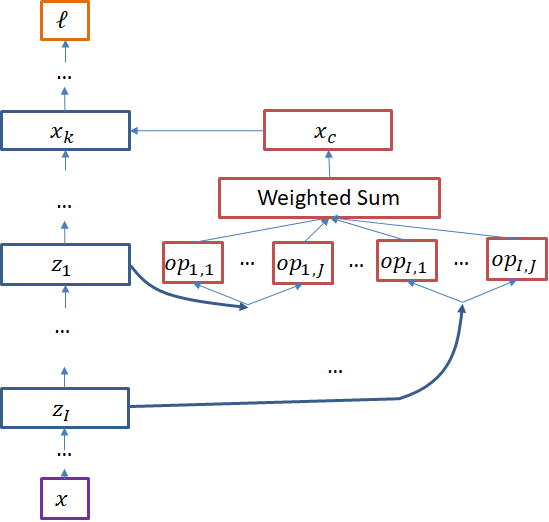
\includegraphics[width=0.44\textwidth, keepaspectratio]{\NASDIR/img/x_c_select.png}
    \label{fig:x_c_select}}
    ~
\subfloat[]{
    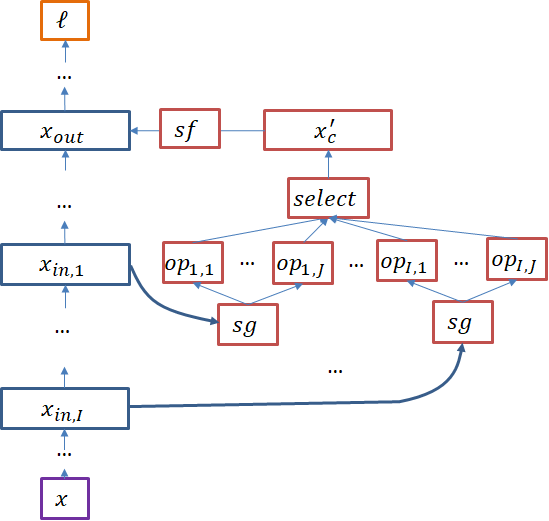
\includegraphics[width=0.44\textwidth, keepaspectratio]{\NASDIR/img/x_c_select_sf_sg.png}
    \label{fig:x_c_select_sf_sg}}
    \caption{Training of a weak learner $x_c$, so that it can (a) and cannot (b) affect the current model.}
\end{figure}

\textbf{Combining Weak Learners.} During the joint weak learning, we initialize a weighted sum of all the the unary operations on all the possible inputs as
\begin{align}
    x_c = \sum _{i=1}^I \sum_{j=1}^J \alpha_{i,j} op_j(z_i),
    \label{eq:x_c_select}
\end{align}
where we enumerate the possible operations as $op_j$ and the possible inputs as $z_i$, and $\alpha_{i,j}$ is the weight of the unary operation $op_j(z_i)$. 
The merge operation of $x_c$ during the joint weak learning is the above weighted sum for simplicity of formulation, and it can be viewed as a special case 
of concat-projection. We will replace this merge operation once we choose the shortcut connections in Sec.~\ref{sec:candidate_finalize}. 

\textbf{$L1$-regularization.} Each $op_j(z_i)$ is normalized with batch-normalization to have zero mean and unit variance in expectation, so that $\alpha_{i,j}$ reflects 
the importance of the operation.
To learn the most important operations, we apply $L1$-regularization~\citep{lasso} on the weight vector $\vec{\alpha}$ to encourage sparsity, i.e.,
we add the following loss during the fitting of $x_c$,  
\begin{align}
    \lambda \Vert \vec{\alpha} \Vert_1 = \sum_{i=1}^I \sum _{j=1}^J | \alpha _{i,j} |,
    \label{eq:x_c_select_loss}
\end{align} 
where $\lambda$ is a hyperparameter. $L1$-regularization, known as Lasso, induces sparsity in the parameter and is widely used for feature selection. It has also been successfully applied to model compression of neural networks such as in~\citep{huang2017condensenet}.


\textbf{Weak learning.} 
The goal of weak learning is to match $x_c$ with the negative gradient of the loss with respect to the layer $x_{k}$, i.e., 
we minimize 
\begin{align}
   \langle \nabla_{x_{k}} \mathcal{L}, x_c \rangle =  
   \langle \nabla_{x_{k}} \mathcal{L}, \sum _{i=1}^I \sum_{j=1}^J \alpha_{i,j} op_j( \stopgradient( z_i ) ) \rangle,
    \label{eq:x_c_linear_loss}
\end{align}
where $\stopgradient$ is short for stop-gradient, and is an operation to treat each $z_i$ as a constant, so that the optimization of weak learners does not 
affect the current network. Mathematically, $\stopgradient(x) = x$ during forward, and has zero gradient with respect to $x$ during backward.

We add the loss~\ref{eq:x_c_linear_loss} implicitly to the overall objective on line~\ref{algline:add_sf}, and an explanation is as follows.
A naive implementation is to add the loss in Eq.~\ref{eq:x_c_linear_loss} to the additional $\ell_{extra}$, and backpropagate the network
while only updating parameters in the weak learners $x_c$. 
However, this will require one to record the intermediate gradients $\nabla _{x_{k}} \mathcal{L}$ during training. 
Interestingly, this can be avoided and it is what we describe in Algorithm~\ref{alg:candidate_init} when $\texttt{is\_frozen}$ is set to true. 
Specifically, on line~\ref{algline:add_sf}, we replace the layer $x_k$ with $x_k + \stopforward(x_c)$, 
where $\stopforward(x_c) = x_c - \stopgradient(x_c)$, so that $\stopforward(x_c) = 0$  during 
forward, and has gradient of identity with respect to $x_c$. As a result, 
for any parameter $\theta$ in weak learner $x_c$ for intermediate layer $x_k$, its gradient during the backpropagation is
\begin{align}
\nabla_{\theta} \mathcal{L} &= \nabla _{x_k + \stopforward(x_c)} \mathcal{L} \nabla _{x_c} \stopforward(x_c) \nabla _{\theta} x_c = \nabla _{x_k}\mathcal{L} \nabla _{\theta} x_c = \nabla_{\theta} \langle \nabla_{x_{k}} \mathcal{L}, x_c \rangle.
\end{align}
This is the same as the gradient of the loss in Eq.~\ref{eq:x_c_linear_loss} with respect to $\theta$.
Hence, exploiting $\stopforward$ and $\stopgradient$ operations on line~\ref{algline:add_sf} and line~\ref{algline:add_sg}, we can
optimize both the current network and the weak learners at the same time without the weak learners affecting the network. Furthermore, 
we do not force the training procedure to record $\nabla_{x_k} \mathcal{L}$ explicitly. 

\textbf{Warm-start.} After appending the weak learners to an existing and trained model, we warm-start the training with the parameters
of the existing model, and initialize the weak-learner parameters randomly. Leveraging these existing models parameters, 
we can potentially spend fewer epochs per model, because we only need to fit the weak learners, which are
shallow networks.

\subsection{\petridishhard versus \petridishsoft Training of Weak Learners}
\label{sec:soft_vs_hard}
An interesting consideration is whether to stop the influence of the weak learners to the models during the weak learning. 
On one hand, we eventually want to add the weak learners into the model and allow them to be backpropagated togther
to improve the model accuracy.
On the other hand, the introduction of 
untrained weak learners to trained models may negatively affect the training. Furthermore, the models may develop dependency on weak-learner shortcuts 
that are not selected, which can also negatively affect the future models. 
To study the effects through an ablation study, we introduce the $\texttt{is\_frozen}$ variable for Algorithm~\ref{alg:candidate_init}. 
When it is false, we replace the occurrence of $\stopforward$ and $\stopgradient$ with identity, so that the weak learners are directly added to the models, 
as illustrated in Fig.~\ref{fig:x_c_select}. We call this variant
\petridishsoft, and we compare it with \petridishhard, where $\texttt{is\_frozen}$ is true, in Sec.~\ref{sec:experiment_soft_vs_hard}. 


%we train and select the candidate layers. On one hand, most of our parent models are partially trained (more detail in Sec.~\ref{sec:candidate_finalize}) and the parent model contributes to the majority of the total computation, so we consider it very wasteful to freeze the parent parameters. On the other hand, if the parent model is frozen, different selection modules become independent of each other and may be easier to learn. Furthermore, freezing parent models prevents the newly initialized candidate layers from negatively affecting the parent model. C2~\citep{cascadecorr} thus adopts freezing the parent. 



\subsection{Weak Learner Finalization}
\label{sec:candidate_finalize}

\begin{figure}[t]
\centering
    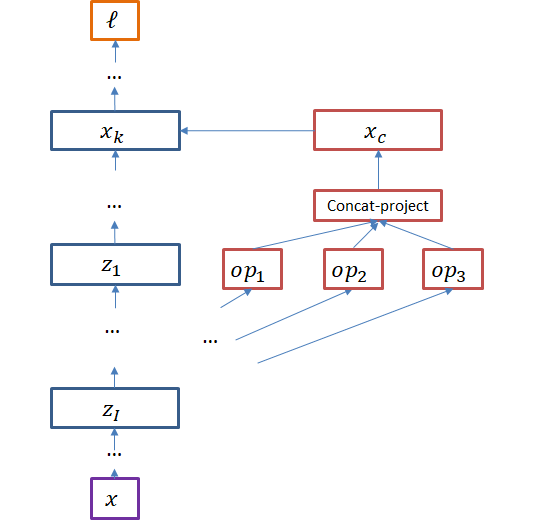
\includegraphics[width=0.44\textwidth, keepaspectratio]{\NASDIR/img/x_c_select_final.png}
    \caption{Weighted sum is replaced with concat-projection, when the top operations are chosen. Any $\stopforward$ or $\stopgradient$ are also removed.}
    \label{fig:x_c_select_final}
\end{figure}

Algorithm~\ref{alg:candidate_select} describes how we select and finalize the weak leaner into the existing models. 
The absolute value of the weights $\alpha_{i,j}$ convey the importance of the associated candidate operations. Upon finishing training the candidate layers with a few epochs, we keep the top $I_{max}$ operations for each selection module in terms of the corresponding $| \alpha _{i,j} |$. 
Other operations are removed. In our experiments in Sec.~\ref{sec:sum_vs_cat_proj}, we found a simple modification to be crucial for the final model cost-efficiency: instead of combining the selected operations in a weighted sum as in the selection phase, we concatenate the feature maps along the feature dimension, and project the result with 1x1 convolution to the same channel size as the target $x_{out}$ before summing them together to replace $x_{out}$, as illustrated in Fig.~\ref{fig:x_c_select_final}. This modification is in fact implicitly used by most of the existing neural architecture search works~\citep{NASCell,Pham2018EfficientNA}, where the layers within a cell is concatenated to form the cell output, and any operations on the output first project it to the same channel size as layers that are not cell outputs. We train the finalized model for a few epochs warm-starting with the parameters from the weak learning phase. 






\subsection{Utilizing Parallel Workers}
\label{sec:parent_choice}


%\begin{algorithm}[t]
%\begin{algorithmic}[1]
%\STATE Set $T = $
%\STATE \textbf{Input}: (1) a pool of trained models, $Q_{p}$; 
%(2) search tree depth for each model $m$, $d(m)$, e.g., the initial model has $d(m) = 0$; 
%(3) number of times each model $m$ is chosen as parents, $n(m)$. 
%\STATE Compute the lower convex hull of the models on the plot of test-time computational costs versus error rates of models. 
%\STATE Sample a model $m$ on the hull, with probability defined by Eq.~\ref{eq:parent_weight}. 
%\STATE \textbf{Output}:  A model $m$ selected as the parent model. 
%\end{algorithmic}
%\caption{Select Parent( )}
%\label{alg:select_parent}
%\end{algorithm}

The proposed iterative architecture growth may be noisy 
due to the randomness during training of weak learners and 
the expanded models. By leveraging parallel workers, we 
can explore multiple growths to find more cost-effective models. 
The parallel workers can share knowledge and expand from any searched models, 
and this section describes their sampling procedure.

We maintain the lower convex hull of the performance of the 
searched models on the validation error versus test-time computation 
graph. The models on the hull are the most cost-efficient, 
because no mixture of other searched models is both more accurate and less expensive
than any of them. To choose one model on the hull, we enter a while-loop
from the most accurate model that is within the computation 
budget $K$ to the least accurate on the hull, 
and sample a model $m$ and exit the loop with probability $1/(n(m) + 1)$, 
where $n(m)$ is the number of times that model $m$ has already been selected. 
This is because the next child model expanded from $m$ is the best among the children with probability
$1/(n(m) + 1)$, assuming the children are uniformly drawn. 
We also favor the more accurate models as it is often more difficult to 
improve an already accurate model. In practice, we explore few 
models totally $(<50)$, so that the effect of different sampling on the hull 
is not clear. We defer a more detailed discussion to Sec.~\ref{sec:appendix_parent_choice}.



    
\section{Experiment}

%%%%%%%%%%%%%%%%%%%%%%%% 
% Experimental questions
%%%%%%%%%%%%%%%%%%%%%%%%
%\subsection{Experimental questions}
%\begin{enumerate}
%\item 
%\end{enumerate}


%%%%%%%%%%%%%%%%%%%%%%%% 
% Data-sets
%%%%%%%%%%%%%%%%%%%%%%%%

%%%%%%%%%%%%%%%%%%%%%%%% 
% Eval metric
%%%%%%%%%%%%%%%%%%%%%%%%
%\subsection{Evaluation Metrics}

%\begin{enumerate}
%    \item For fixed search space and training parameters, we can 
%    compare the best found model validation error after the same number of 
%    models are trained.
    %\item For a more general comparison among search algorithms, we plot the curves of the best validation error versus FLOPs spent on training. Then the lower curves represent algorithms that find the most accurate models faster.
    %\item While the previous two metrics focus on how fast the search can find the most accurate models, they do not consider the cost-efficiency of the searched models. To evaluate the cost-efficiency, we represent the cost-efficiency of searched models by the lower convex hull of validation error versus model computational cost, measured in FLOPs. The more close the hull is to the origin, the more cost efficient the found models are. We can compare algorithms by comparing their performance convex hulls. 
%\end{enumerate}


%%%%%%%%%%%%%%%%%%%%%%%% 
% Parent choice Experiment
%%%%%%%%%%%%%%%%%%%%%%%%


%%%%%%%%%%%%%%%%%%%%%%%% 
% Visual Recognition Data-sets
%%%%%%%%%%%%%%%%%%%%%%%%
\subsection{Search Results on CIFAR10}
\label{sec:experiment_cifar10_search}

\textbf{Set-up.}
We first apply the proposed algorithm to search for architectures on CIFAR-10~\citep{cifar}. During search, we use a fixed set of 45000 training images for training, and 5000 for validation. Both weak learner initialization and finalization are trained for 80 epochs, with a batch size 32 and a learning rate that decays from 0.025 to 0 in cosine decay~\citep{cosine_lr}. We apply drop-out~\citep{larsson2016fractalnet} and cut-out~\citep{cutout} during search. The final found model is trained from scratch using the same parameters, except that it trains on all 50000 training images, and spends 600 epochs. 


\textbf{Search Results.} 
Table~\ref{tab:cifar10_search} depicts the test-errors, model parameters, and search computation of the proposed methods along with many state-of-the-art methods.
\Petridish cell search finds a model with 2.61\% error rate with 2.5M parameters, in 5 GPU-days, which is at  state-of-the-art level. \Petridish macro search finds a model that achieves 2.86\% error rate using 4.8M parameters in 27.2 GPU-days . This is significantly better than any previous macro search results, 
and showcases that macro search can find cost-effective architectures that are previously only found through cell search. 

\textbf{Importance of initial models.}
Table~\ref{tab:cifar10_search} also showcase the impact of initial models to the final results of architecture search. This is an important topic, because existing literature has been moving away from macro architecture search, as early works~\citep{NASCell,Pham2018EfficientNA,Real2018RegularizedEF} have shown that cell search results tend to be superior than those from macro search. However, this result may be explained away by the superior initial models of cell search: the initial model of \Petridish is one of the simplest model that any of the listed cell search methods would propose and evaluate, and it already achieves 4.6\% error rate using only 0.4M parameters, a result that is on-par or better than many macro search results. 


\begin{table*}[t]
    \centering
    \caption{Comparison against state-of-the-art recognition results on CIFAR-10. Results marked with $\dagger$ are not trained with cutout. The first block represents approaches for macro-search. The second block represents approaches for cell-search. 
    }
    \begin{tabular}{l|cccc}
    \hline
\multirow{ 2}{*}{\textbf{Method} }
        &  \textbf{\# params} 
        &  \textbf{Search } 
        &  \textbf{Test Error } \\
        &  (mil.)
        &  (GPU-Days)
        &  (\%)\\
\hline
\citet{nas}$^{\dagger}$
    &  7.1 &  1680+ &  4.47  \\
\citet{nas} + more filters$^{\dagger}$
    &  37.4 &   1680+ &  3.65   \\
\citet{Real2017EvoNet}$^{\dagger}$
    &  5.4 &   2500 &  5.4  \\
ENAS macro~\citep{Pham2018EfficientNA}$^{\dagger}$
    &  21.3 &  0.32 &  4.23 \\
ENAS macro + more filters$^{\dagger}$
    &  38 &   0.32 &  3.87 \\
Lemonade I~\citep{Elsken2018EfficientMN}
    &  8.9 &    56 &  3.37 \\
\hline
\Petridish initial model ($N=6$, $F=32$)
    & 0.4 &  -- & 4.6 \\
%\Petridish macro without DropPath
%    & 3.1 & 6 & 3.38 \\
\textbf{\Petridish macro} 
    & \textbf{2.2} & 5 & \textbf{2.83} \\
%\Petridish macro (start at $N$=3, $F$=32)
%    & 2.7 & 18 & 3.44 \\
\hline \hline
NasNet-A~\citep{NASCell}
    &  3.3 &    1800 &  2.65   \\
AmoebaNet-A~\citep{Real2018RegularizedEF}
    &  3.2 &  3150 &  3.3  \\
AmoebaNet-B~\citep{Real2018RegularizedEF} 
    &  2.8 &   3150 &  2.55 \\ 
PNAS~\citep{Liu2017ProgressiveNA}$^{\dagger}$
    &  3.2 &  225 &  3.41 \\
Heirarchical NAS~\citep{Liu2018HierNA}$^{\dagger}$
    &  15.7 &    300 &  3.75 \\ 
ENAS cell~\citep{Pham2018EfficientNA}
    &  4.6 &  0.45 &  2.89 \\ 
ENAS cell~\citep{Pham2018EfficientNA}$^{\dagger}$
    &  4.6 &  0.45 &  3.54 \\ 
Lemonade II~\citep{Elsken2018EfficientMN}
    &  3.98 &  56 &  3.50 \\
Darts~\citep{Liu2018DARTSDA}
    &  3.4 &   4 &  2.83 \\ 
Darts random~\citep{Liu2018DARTSDA}
    & 3.1 & -- & 3.49 \\
\citet{CaiPathLevel} 
    & 5.7 &  8  & 2.49 \\
\citet{NAONet}$^{\dagger}$
    & 3.3 & 0.4 & 3.53 \\
\hline
\textbf{\Petridish cell}
    & \textbf{2.5} & 5 & \textbf{2.61} \\
%\Petridish cell + more filters
%    & 3.5 & 6 & 3.05 \\
\hline
    \end{tabular}
    \label{tab:cifar10_search}
\end{table*}



\subsection{Transfer to ImageNet}
\label{sec:experiment_vision_transfer}



\begin{table*}[t]
    \centering
    \caption{ILSVRC2012 transfer results. \Petridish uses \petridishhard and the concat-projection (CP) modification by default. 
    }
    \begin{tabular}{l|cccc}
    \hline
\multirow{ 2}{*}{\textbf{Method} }
        &  \textbf{\# params} 
        &  \textbf{\# multi-add}
        &  \textbf{Search}
        &  \textbf{top-1 Test Error } \\
        &  (mil.)
        &  (mil.)
        &  (GPU-Days)
        &  (\%)\\
\hline
Inception-v1 (Szegedy et al., 2015)
    & 6.6 & 1448 & -- & 30.2 \\
MobileNetV2 (Sandler et al., 2018)
    & 6.9 & 585 & -- & 28.0 \\
\hline
NASNet-A (Zoph et al., 2017) 
    & 5.3 & 564 & 1800 & 26.0 \\
NASNet-B (Zoph et al., 2017) 
    & 5.3 & 488 & 1800 & 27.2 \\
AmoebaNet-A (Real et al., 2018)
    & 5.1 & 555 & 3150 & 25.5 \\
PNAS (Liu et al., 2017a)
    & 5.1 & 588 & 225  & 25.8 \\
DARTS (Liu et al., 2018)
    & 4.9 & 595 & 4    & 26.9 \\
\hline
\textbf{\Petridish macro} (F=32) %828
    & 4.9 & 593 & 27.2 & 29.4 \\
\textbf{\Petridish macro} (F=48) %822
    & 10.4 & 1247 & 27.2 & 25.2 \\
\hline
\textbf{\Petridish cell} (F=40) %1172
	& 3.2 & 500 & 5 & 27.0 \\
\textbf{\Petridish cell} (F=44) %1180 
    & 4.8 & 598 & 5 & 26.0 \\
\hline
\end{tabular}
\label{tab:imagenet_compare}
\end{table*}





For ILSVRC2012~\citep{ILSVRC15}, we take the standard data augmentation approach of~\citep{resnet}, and use 224x224 input images. To utilize the found architecture that are designed for 32x32 images, we apply a 3x3 conv with stride 2 to transform the RGB-color into $F / 4$ channels, and then apply two transition cells (as stated in Sec.~\ref{sec:candidate_init_and_select}) to down-sample the feature map to 28x28 and $F$ channels. We treat the resulting tensor as the input image for the found architectures. 

The top-1 error rate, the number of model parameters and the test-time computational cost in terms of mult-adds are shown in Table~\ref{tab:imagenet_compare}. Model of \Petridish cell-search achieves 26.0\% error rate using 4.8M parameters and 598M multi-adds, which is on par with state-of-the-art results listed in the second block of Table~\ref{tab:imagenet_compare}. By utilizing feature selection techniques to evaluating multiple model expansions at the same time, \Petridish is able to find models faster by one or two orders of magnitudes than early methods that train models independently, such as NASNet~\citep{NASCell}, AmoebaNet~\citep{Real2018RegularizedEF}, and PNAS~\citep{Liu2017ProgressiveNA}.  
In comparison to super-graph methods such as DARTS~\citep{Liu2018DARTSDA}, \Petridish cell-search sacrifices about four times search speed for the flexibility to grow from existing models. 

We also observe that the model from \Petridish macro-search achieves 29.4\% error rate using 4.9M parameters and 593M multi-adds, a comparable result to the human-designed models in the first block of Table~\ref{tab:imagenet_compare}. To the best of our knowledge, this is one of the first successful result to transfer macro-search results on CIFAR to ImageNet, showing that macro-search results can be transferred. 
However, we do observe the gap in error rates between \Petridish macro from \Petridish cell, suggesting that giving full freedom of choosing input layers as in \Petridish macro may reduce the search speed to find a state-of-the-art model.


\subsection{Weighted Sum versus Concatenation-Projection}
\label{sec:sum_vs_cat_proj}



\begin{table}[t]
    \centering
    \caption{ILSVRC2012 transfer results. 
    	Ablation study on the choice of weighted-sum (WS) versus concat-projection (CP) as the merge operation in finalized weak learners.
    	The search were with parameter initial channel $F=32$ and number of regular cell per resolution $N=6$. 
    }
    \begin{tabular}{l|cccc}
    \hline
\multirow{ 2}{*}{\textbf{Method} }
        &  \textbf{\# params} 
        &  \textbf{\# multi-add}
        &  \textbf{Search}
        &  \textbf{top-1 Test Error } \\
        &  (mil.)
        &  (mil.)
        &  (GPU-Days)
        &  (\%)\\
\hline
WS macro(F=48) %808
    & 5.9 & 756 & 29.5 & 32.5\\
CP-end macro (F=36) %845
    & 5.4 & 680 & 29.5 & 29.1 \\
{CP macro} (F=32) %828
    & 4.9 & 593 & 27.2 & 29.4 \\
\hline
WS cell (F=48) %810
    & 3.3 & 477 & 22.8 & 32.7\\
CP-end cell  (F=44) %848
    & 4.7 & 630 & 22.8 & 27.2 \\
\textbf{CP cell} (F=40) %841
    & 4.4 & 583 & 15.3 &  26.9 \\
\hline  
\end{tabular}
\label{tab:imagenet_ws_vs_cp}
\end{table}



After selecting the operations in Sec.~\ref{sec:candidate_finalize}, we concatenate them and project the result with 1x1 conv so that the result can be added to the output layer $x_{out}$. 
Here we empirically justify this design choice.

We first consider applying the switch only to the final reported model, i.e., we do not use concat-project as the merge operation during search, and only switch all weak learner weighted-sums to concat-projections in the final model, which we train from scratch to report results. We call this variant CP-end, and the variant where we never switching to concat-projection as WS. Since concat-projection incurs additional computation to the model, we increase the channel size of WS variants so that the two variants have similar test-time multi-adds for fair comparisons. The default \Petridish option is switching the weak learner weighted-sums to concat-projections at each time weak learners are finalized, we name it CP. We compare WS, CP-end and CP on the transfer results on ImageNet in  Table~\ref{tab:imagenet_ws_vs_cp}, and we observe that CP is better in the sense that it achieves better or similar prediction error using less test-time computation and training-time search. 



\subsection{\petridishhard versus \petridishsoft}
\label{sec:experiment_soft_vs_hard}

\begin{table}[t]
    \centering
    \caption{ILSVRC2012 transfer results. 
    	Ablation study on the choice of \petridishsoft and \petridishhard for training the weak learners. 
    	The search were with parameter initial channel $F=32$ and number of regular cell per resolution $N=6$. 
    }
    \begin{tabular}{l|cccc}
    \hline
\multirow{ 2}{*}{\textbf{Method} }
        &  \textbf{\# params} 
        &  \textbf{\# multi-add}
        &  \textbf{Search}
        &  \textbf{top-1 Test Error } \\
        &  (mil.)
        &  (mil.)
        &  (GPU-Days)
        &  (\%)\\
\hline
\Petridish \petridishsoft cell (F=32) %843,842,833,834
    & 4.0 & 546 & 20.6 & 32.8 \\
\textbf{\Petridish \petridishhard cell} (F=40) %841
    & 4.4 & 583 & 15.3 &  26.9 \\
\hline
\end{tabular}
\label{tab:imagenet_soft_vs_hard}
\end{table}


In Sec.~\ref{sec:soft_vs_hard}, we apply $\stopforward$ and $\stopgradient$ to block the influence of feature selection modules to the parent models. We call this default version \petridishhard. 
We compare this against \petridishsoft, where $\stopforward$ and $\stopgradient$ are simply replaced with identity so that the weak learners are directly inserted into the model. Table~\ref{tab:imagenet_soft_vs_hard} showcases the transfer results of \petridishhard  and \petridishsoft to ImageNet. We compare \Petridish cell (F=40) with \petridishsoft cell (F=32), two models that have similar computational cost but very different accuracy, and we observe that \petridishhard leads to much better model than \petridishsoft for cell-search. 


\section{Discussion}
\label{sec:discussion}
Since the NAS problem is a combinatorial optimization, we have to approach it with either better approximation algorithms, or utilize the special conditions of the search space itself. 
In particular, a search space on CIFAR10 is studied by~\citep{nasbench}, which shows that architectures that are similar also have similar statistical performances. 
This suggests that a local search where models are changed iteratively and gradually can be very efficient if the starting model is already near the optimal model.
Luckily this can often be the case. The benchmark results concludes that the best human designed models such as Resnets, DenseNet, and Inception, are all close to 
the pareto frontier of the computation versus error plot, so that these models are naturally good starting points, as evidenced by this work. 



\section{Conclusion}
\label{sec:conclusion}
In this work, we formulate the neural architecture search problem (NAS) as a bi-level optimization problem, which also generalizes the anytime linear prediction problem. 
Interestingly, existing works often approach this problem with exhaustive search, backward elimination and sparse optimization approaches. 
Instead, we propose an approach that is inspired by gradient boosting to expand intermediate layers iteratively, which mimic forward selection, and least-angle regression 
in particular for feature selection in linear predictions. We also speed up the training of the weak learners by jointly training the union of all possible weak learners,
and at the same time learn to select the most influential subset to form the final weak learner. We demonstrate the search on CIFAR10 and transfer the result to ILSVRC2012,
and we show that this iterative approach is capable of finding state-of-the-art level models using small number of GPU-days.
%\bibliographystyle{sty_bst/icml.bst}
%\bibliography{network_search}

\appendix
\section{Additional Details on Choosing Parent Models}
\label{sec:appendix_parent_choice}
\subsection{Intuitions}
\label{sec:candidate_parent_intuition}

To choose models on the convex hull in a fair manner, we have the following intuitions.
\begin{enumerate}
\item 
Since we want to maximize the improvement of the pareto front per unit cost spent during training, we should discount the probability of a model to be chosen, $p(m)$, by the cost of the model $c(m)$, which is proportional to the training cost.
\begin{align}
    p(m) \propto \frac{1}{c(m)}
\end{align}

\item 
In Sec.~\ref{sec:candidate_init_and_select}, we choose a number of input layers for each selection modules. The number of possible inputs is $d(m) + 2$, the editing distance from the current model $m$ to the seed model. Among them, we choose $\eta d(m)$ as input layers, where $\eta$ is a constant in $(0,1]$ deciding the growth rate of the model. 
Hence, each cell in model $m$ has ${ d(m) + 2 \choose \eta d(m) }$ possible selection modules to be attached with. 

In cell search, there are two free cells, normal and reduction cells. In macro search, every cell is free, and in the case of visual recognition, there are 20 cells. Let $f(m)$ be the number of free cells in the model $m$. Then we should sample a model with a number of times that is proportional to its possible selection modules, in order to uniformly sample all models uniformly at random. Hence, we have

\begin{align}
    p(m) \propto { d(m) + 2 \choose \eta d(m) } ^{f(m)}.
\end{align}



\item 
When we have chosen a model $m$ for $n(m)$ times, we should sample it with probability discounted by a factor $\frac{1}{n(m) + 1}$, because assuming uniformly sampling possible children models, the next one is the best with a probability $\frac{1}{n(m) + 1}$
\begin{align}
    p(m) \propto \frac{1}{n(m) + 1}
\end{align}

\item 
\citet{Elsken2018EfficientMN} use inverse of probability density to sample the models, where the density function is based on the model parameter sizes. This also supports the intuition that 
when models are clustered together, i.e., having similar computational cost, and/or accuracy, we should discount their probability, because they only represent a small portion of the convex hull. 
To compute the probability density at the computational cost of model $m$, we use non-parameter regression with the points on the convex hull. E.g., we can use Gaussian kernel with the median distance as the kernel width to estimate the density as $pdf(c(m))$. Then we weight the probability of choosing $m$ as the parent with 
\begin{align}
    p(m) \propto \frac{1}{pdf(c(m))}
\end{align}

\item

As models grow larger and and more accurate, we expect to have smaller fraction of candidate expansion to be able to positively affect the accuracy and/or cost-effectiveness of the model. Hence, we may want to sample the larger and/or more accurate models more often than the early and inaccurate models, in order to achieve uniform improvement of the convex hull. If the fraction of beneficial candidate expansions $b(m)$ is a constant, then item (2) above already addresses this problem. If the fraction is indeed decreasing, then we need to set $p(m)$  inversely proportional to this fraction, i.e.,
\begin{align}
    p(m) \propto \frac{1}{b(m)}.
\end{align} 
However, this is difficult to achieve, because $b(m)$ cannot be estimated and $b(m)$ can be zero. 

A workaround to estimate $b(m)$ is with the proportion of children of the parent of $m$ that we have sampled before finding $m$, $\tilde{b}(m)$. This is also a work around for the problem of $b(m) = 0$, because by finding $m$, the parent of $m$ definitely has non-zero $b()$. 
Hence, we instead have 
\begin{align}
    p(m) \propto \frac{1}{\tilde{b}(m)}.
\end{align}

\end{enumerate}


\subsection{Possible Algorithms}

\subsubsection{Greedy Expansion}
\todo{This is proposed by John in email chain Jan 22.}
The algorithm is as follows.
\begin{enumerate}
    \item Sort the models in the order of their error rates in increasing order as $m_1, m_2,...$
    \item While we have not chosen a model, we loop with $i =1,2,3,$ and so on. For each $i$, we choose $m_i$ with probability $p(m_i) = \frac{1}{n(m_i) + 1}$. 
\end{enumerate}

\subsubsection{Intuition Kitchen Sink}
Combining the intuitions of Sec.~\ref{sec:candidate_parent_intuition}, we have the probability to choose model $m$ to be 
\begin{align}
    p(m) \propto \frac{ {d(m) + 2 \choose \eta d(m) }^{f(m)} }{pdf(c(m)) c(m) (n(m) + 1) \tilde{b}(m)  }.
\end{align}




%\end{document}
